\section{Task 2 - Simulating the Bosch process}
The Bosch- or DRIE-etch process is a method to create deep trenches or shappes
with high aspect ratios. Such structures can be used for integrated capacitors or memory devices.

For this task the "drilling" of a circular hole into a substrate is examined.

\subsection{Initial setup}
The Bosch process requires an initial hole in the mask which has to be created by some process as well.
However for this task we assume a perfect cylindrical hole already exists.

We can create the initial layout by stacking a substrate box and a mask box while taking the relative complement with the latter
\begin{figure}[h]
    % Rigth image
    \begin{subfigure}{0.45\textwidth}
    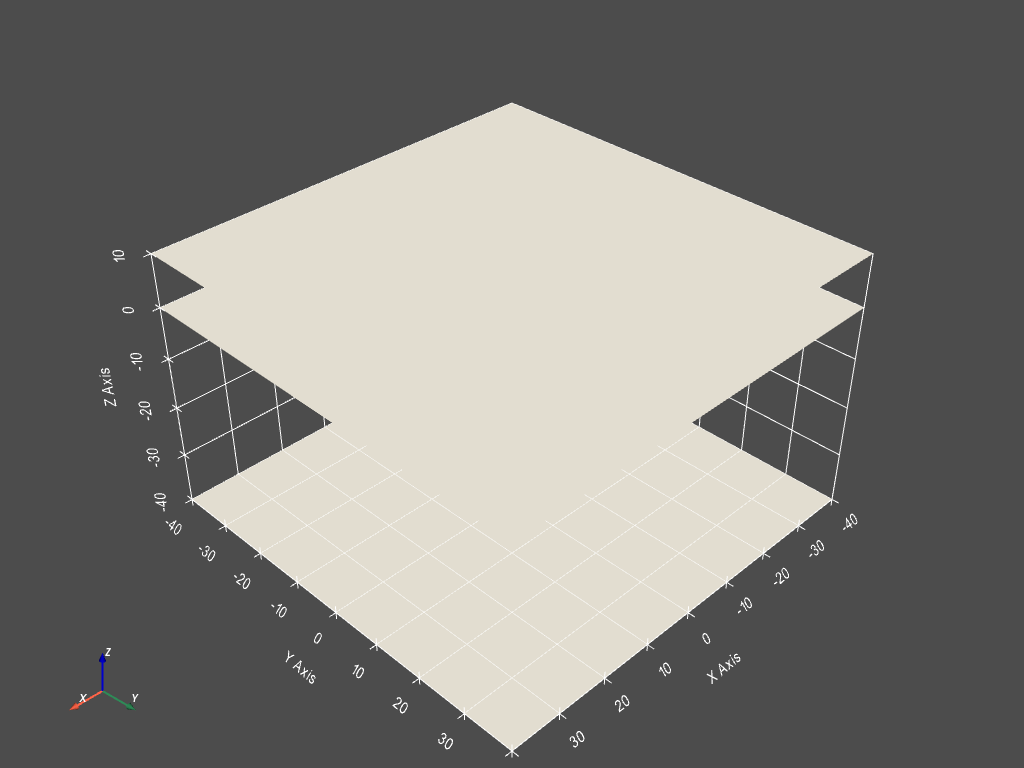
\includegraphics[width=1\linewidth]{res/task2.2_mask.png} 
    \caption{Applying a Mask}
    \label{fig:serial-solution}
    
\end{subfigure}
    % left image
    \begin{subfigure}{0.45\textwidth}
    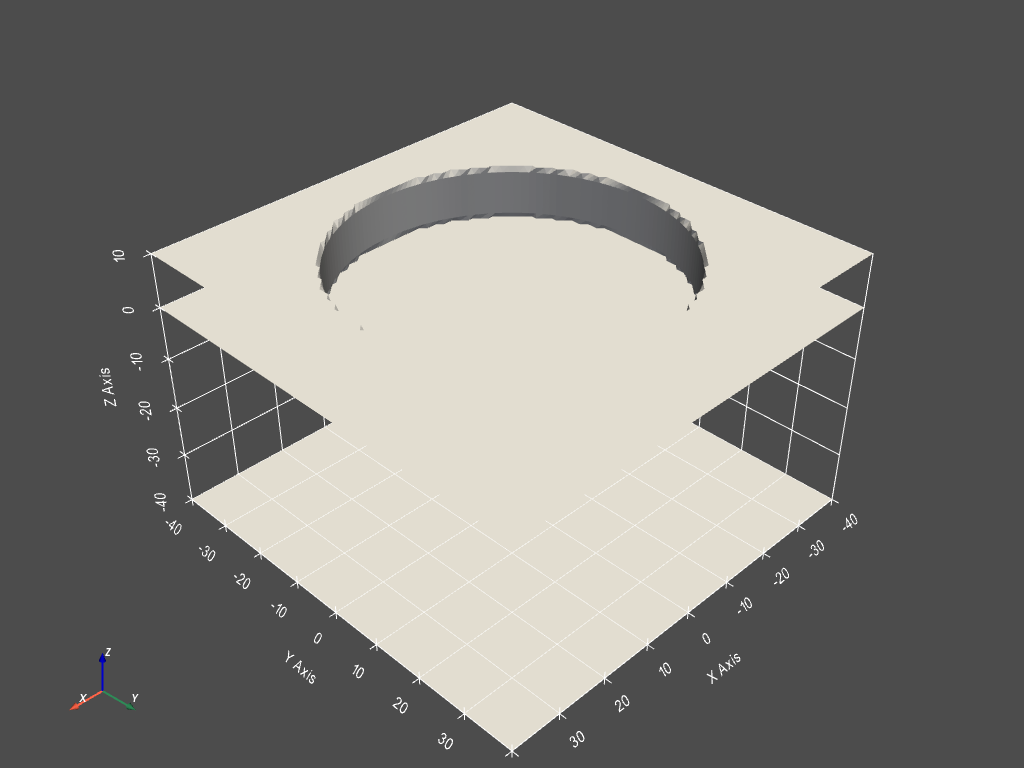
\includegraphics[width=1\linewidth]{res/task2.2_circularHole.png}
    \caption{Cutting a circular hole}
    \label{fig:parallel-solution}
\end{subfigure}

\caption{Creating the initial setup. Mask and substrate appear as planes due to the usage of reflective and infinite boundary conditions}
\label{fig:serial-vs-parallel}
\end{figure}


\subsection{Simulation process}
The process is simulated by performing an initial etch into the substrate followed by 
10 passivation-etch cycles. Substrate etching and passivation is performed uniformly. 
The passivation layer is etched directionally (rate is multiplied by the z-component of the surface normal)

Additionally a randomness factor is introduced to simulate imperfect etching of substrate and and passivation layer.
This is performed by adding a random number from a normal distribution with mean = 0 to the etch rate of all materials as shown in Alg. \ref{cod:etch-field}

\begin{minipage}{\linewidth}
\begin{lstlisting}[caption=etch velocity field, label=cod:etch-field]
double getScalarVelocity(const std::array<double, 3> & /*coordinate*/,
    int material,
    const std::array<double, 3> &normalVector,
    unsigned long /*pointId*/) {
        // if the surface of material 1 is facing upwards, etch it anisotropically
        double vel;
        switch(material)
        {
            case 0:     
                return 0;   // Mask

            case 1:     // substrate
                vel = (-1.)*m_velocity_substrate;
                vel += vel*m_randomNess*distribution(generator);
                return vel;

            default:    // passivation layer
            if(normalVector[2] > 0 )
            {
                vel = (-1)*m_velocity_passivationLayer*std::abs(normalVector[2]);
                vel += vel*m_randomNess*distribution(generator);
                return vel;
            }
            else
            {
                return 0;
            }
        }
    }        
}

\end{lstlisting}
\end{minipage}


Since the mean value of the normal distribution is placed at x=0 both a local increase and decrease in etch rate is possible.
This can be used to model effects such as:
\begin{itemize}
    \item locally increased etch rate caused by particles "breaking off" due mechanical stress such as vibrations
    \item locally decreased etch rate caused by residue being deposited on surface or gas bubbles
    \item crystal granularity if the material is no monocrystal
    \item crystal defects
\end{itemize}


For the purpose of this simulation the deviation from the mean is modelled using a symmetric gauss distribution.

The simulation is set up such that the following parameters are available:
\begin{itemize}
    \item etch time: time in seconds the wafer is submerged in acid
    \item etch velocitry passivation layer: rate at which the passivation material is removed.
    \item etch velocity substrate: rate at which substrate is removed
    \item deposition time: thickness of the passivation layer
    \item steps: number of etch-passivation cycles after the initial etch
    \item randomness: standard deviation of the gauss distribution described above. Random etch rates are calculated relative to the base etch rate. I.e. If the substrate is etched twice as fast the standard deviation is twice as big.
\end{itemize}

\subsection{Results}
The following section shows a selection of possible simulation results with uniform and randomized etch rates after 10 process steps.
The caption below each image shows the simulation parameters which correspond to the listing above.
A quarter of the simulation domain is cut away in order to make the inside of the hole better visible.
Axis units are in nano meters.
\begin{figure}[h]
    % Rigth image
    \begin{subfigure}{0.45\textwidth}
    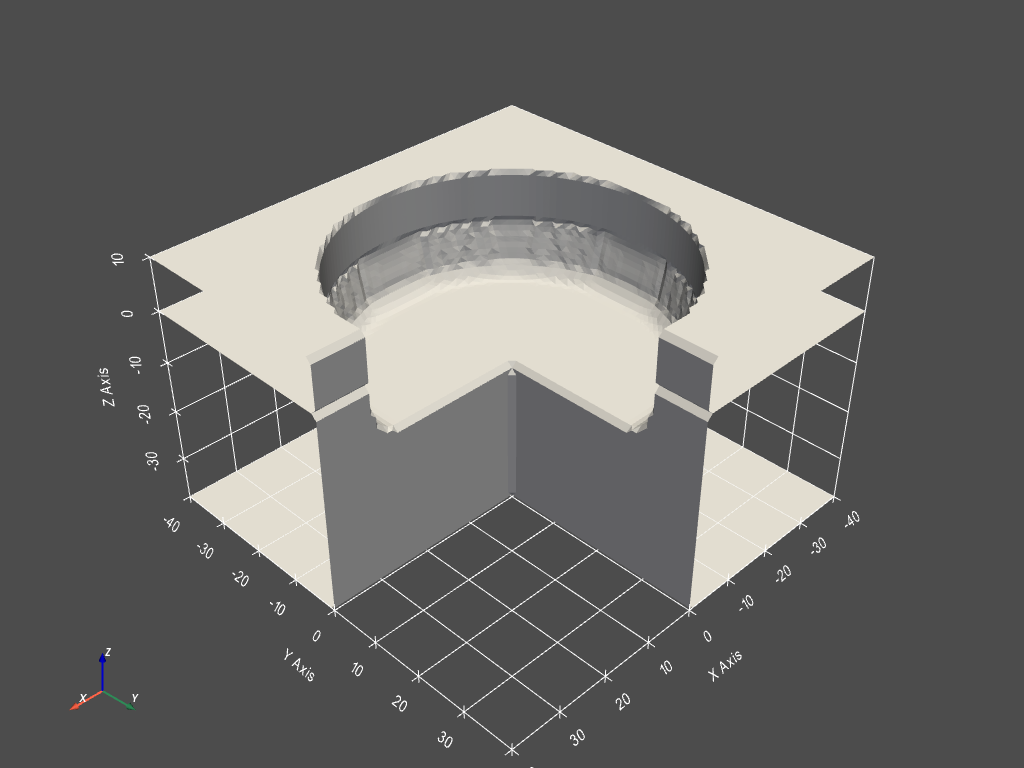
\includegraphics[width=1\linewidth]{res/task2.2_uniformShort.png} 
    \caption{1.5, 1, 0.5, 2.5, 10, 0}
    
\end{subfigure}
    % left image
    \begin{subfigure}{0.45\textwidth}
    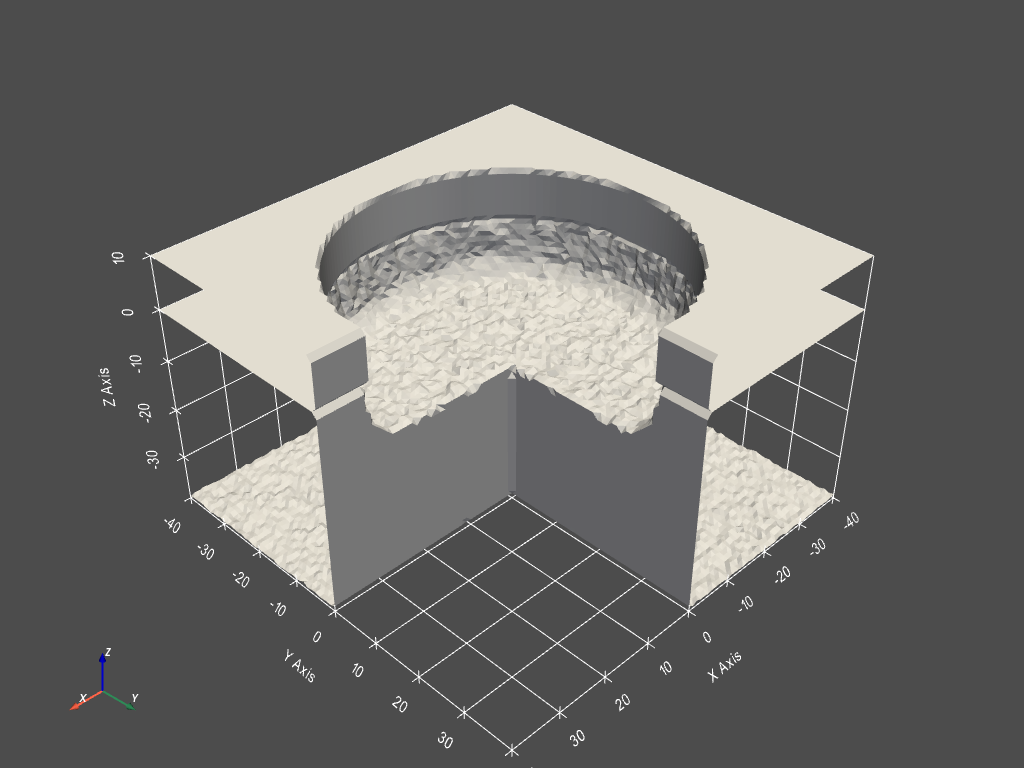
\includegraphics[width=1\linewidth]{res/task2.2_randomShort.png}
    \caption{1.5, 1, 0.5, 2.5, 10, 0}
\end{subfigure}

\caption{Short etchrate. Walls are smoother and single scallops are barely visible}
\end{figure}


\begin{figure}[h]
    % Rigth image
    \begin{subfigure}{0.45\textwidth}
    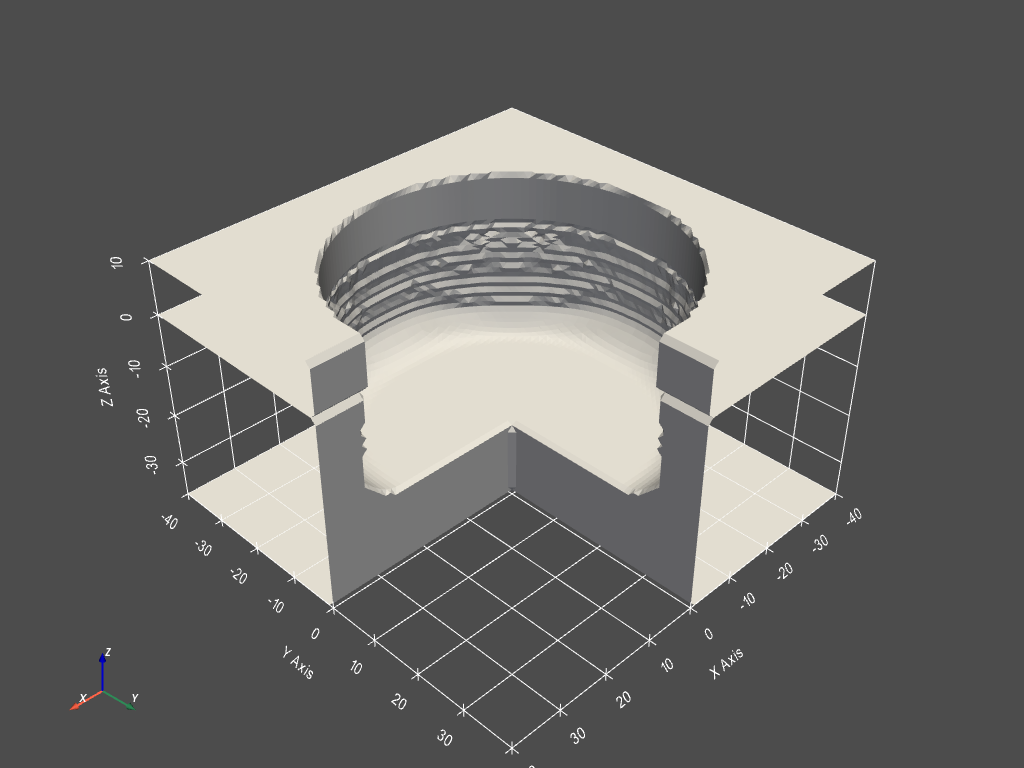
\includegraphics[width=1\linewidth]{res/task2.2_uniformLong.png} 
    \caption{3, 1, 0.25, 2.5, 10, 0}
    
\end{subfigure}
    % left image
    \begin{subfigure}{0.45\textwidth}
    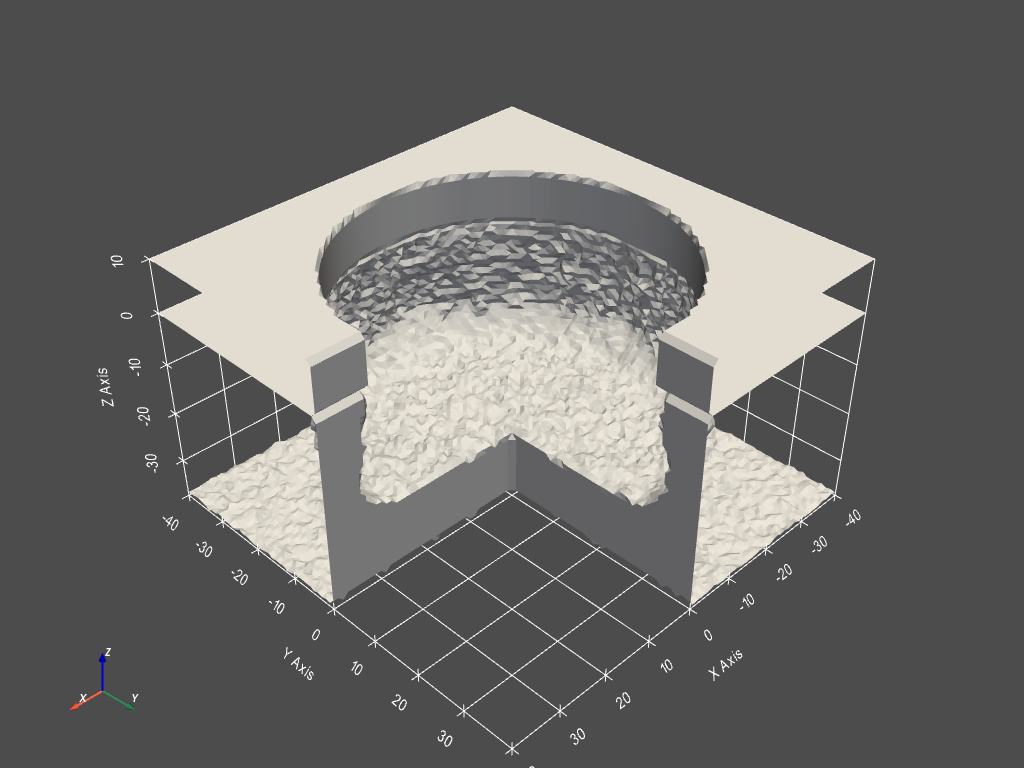
\includegraphics[width=1\linewidth]{res/task2.2_randomLong.png}
    \caption{3, 1, 0.25, 2.5, 10, 0.4}
\end{subfigure}

\caption{Longer etchrate. The hole is significantly deeper but grooves are clearly visible. The randomness blurs "smears" out the grooves but can also create random cavities on the wall}
\end{figure}


\begin{figure}[h]
    % Rigth image
    \begin{subfigure}{0.45\textwidth}
    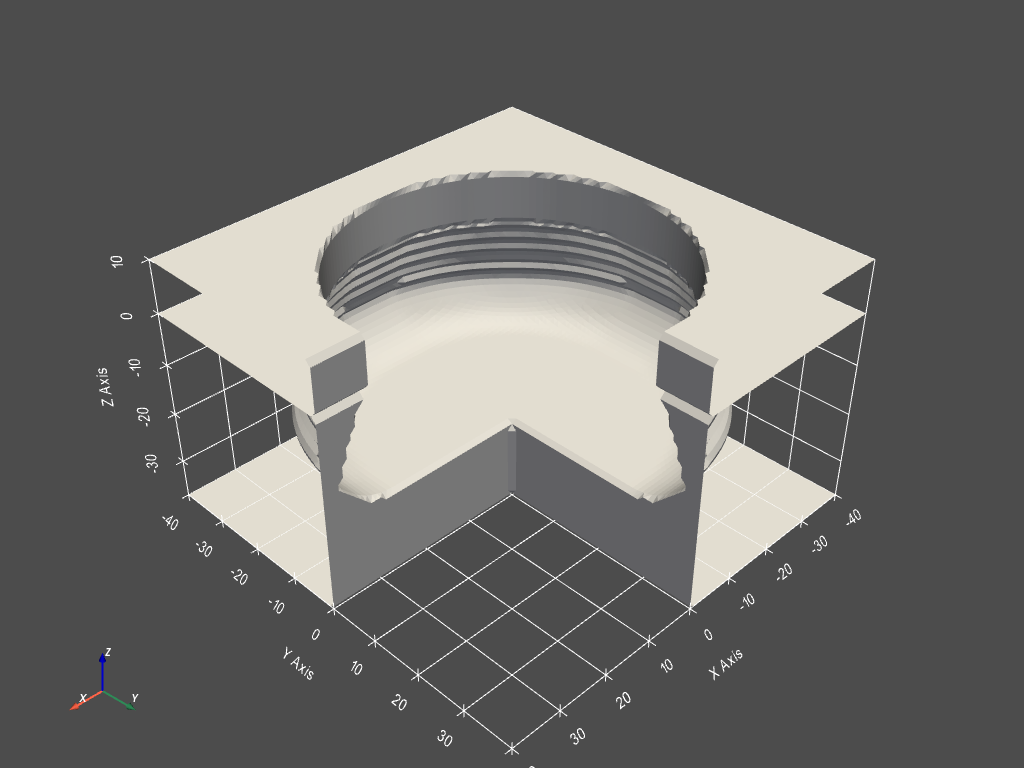
\includegraphics[width=1\linewidth]{res/task2.2_uniformSkewed.png} 
    \caption{2.5, 1, 0.5, 2.5, 10, 0}
    
\end{subfigure}
    % left image
    \begin{subfigure}{0.45\textwidth}
    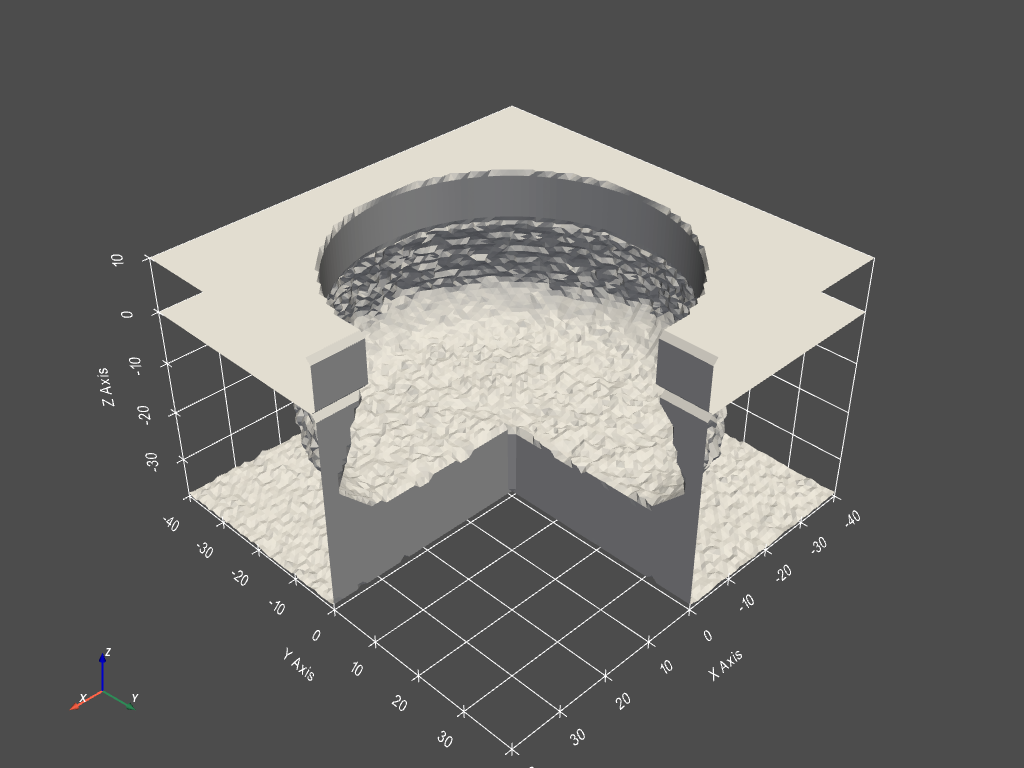
\includegraphics[width=1\linewidth]{res/task2.2_randomSkewed.png}
    \caption{2.5, 1, 0.5, 2.5, 10, 0.4}
\end{subfigure}

\caption{Deep holes but with unbalanced etch and deposition rates. Walls are clearly skewed}
\end{figure}

\subsection{Discussion}
In general it is rather difficult to balance etch- and deposition-rates such that the resulting
wall structure is vertical. This becomes even harder with real materials where rates cannot be arbitrarily set but are defined by the properties of the chosen material.

Depth and wall roughness can best be controlled by adjusting the etch time. While longer etch times can remove more material in each process step the texture of the wall becomes increasingly rough.
Adding randomness to the simulation may smear the edges out by a bit but can also result in bigger random cavities which may have a negative impact on the structural integrity 
if the material is exposed to vibrations or surface tensions during a wet process step.
A rough surface may also be useful for certain applications where a big surface area is needed. 
\begin{figure}[H]
	\centering
	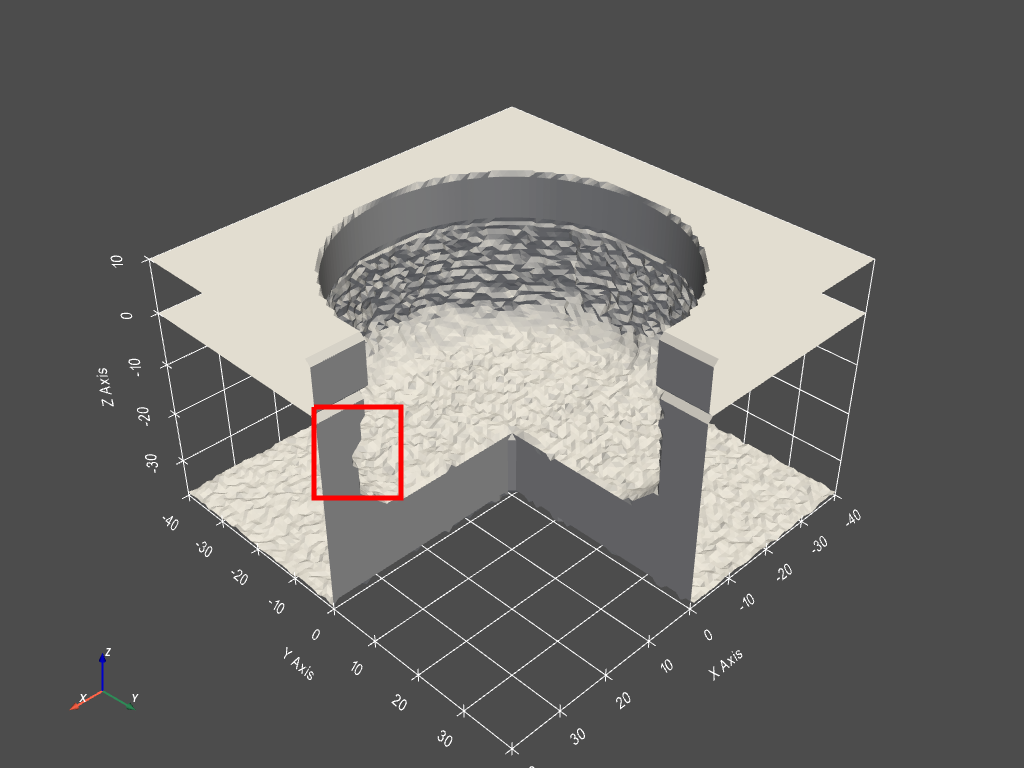
\includegraphics[width=0.75\textwidth]{res/task2.2_cavityBig.png}
	\caption{An example of a bigger random cavity}
\end{figure}

While this process may allow for the creation of structures with high apsect rations it is also very expensive in terms of processing steps.
In addition to etching and deposition further intermediary steps such as cleaning/flushin and quality control are needed (although maybe not between every step)
to achieve good yields. All of these steps are usually performed on different machines.

